\chapter{Implementació}
\label{chap:implementacio}

La implementació del joc s'ha estructurat en dos grans blocs: el servidor i la interfície client. El servidor es l'encarregat de gestionar la informació relativa a les partides disponibles, els jugadors connectats i tota la lògica referent a les partides. La interfície client s'encarrega de interaccionar amb el servidor i mostrar la informació al usuari. 

Per l'intercanvi de dades entre el servidor i el client s'utilitza el protocol WebSocket\footnote{Veure Capítol \ref{sec:websockets}},  ja que ens proporcionen un canal de comunicació bi-direccional. Aquest canal ens permet que els servidor notifiqui al client cada vegada que es produeix un esdeveniment a la partida en curs i que el client notifiqui al servidor les accions que ha dut a terme el jugador. 

\section{Servidor}

El servidor s'encarrega de les següents tasques: 

\begin{itemize}
\item{Proporcionar un servidor web encarregat de servir el programa client per a cada connexió.}
\item{Emmagatzemar les partides en curs i jugadors connectats. Proporcionar esdeveniments a través de WebSockets per a que els usuaris puguin interaccionar a través del programa client. }
\item{Aplicar les regles de la botifarra a cada joc en curs i interactuar amb els diferents clients connectats a una partida}
\end{itemize}

En les properes seccions s'explica més profundament com s'ha realitzat la implementació de cadascuna de les tasques. 

\subsection{Servidor Web}

El servidor web és el procés més important de tot el projecte, ja que és l'encarregat de servir les altres parts de tot el projecte. 

Per la implementació del servidor web s'ha utilitzat el paquet express\footnote{\url{http://expressjs.com/}}. Aquest paquet ens permet desenvolupar servidors web a amb poques línies de codi. Així també disposa de codi pre-programat per tal de realitzar tasques comunes a tots el servidors web. Alguns exemples en són:

\begin{itemize}
\item{Registre de peticions.}
\item{Servir fitxers estàtics (imatges, CSS, JavaScript,etc.).}
\item{Gestió d'errors}
\item{Gestió de galetes (Cookies).}
\end{itemize}

A part de totes aquests funcionalitats, express també s'integra amb diferents llenguatges de plantilles per simplificar l'escriptura del codi HTML. Alguns exemples de motors de plantilles suportats per express són: 

\begin{description}
\item[Haml] {Implementació de Haml\footnote{\url{http://haml-lang.com/}} }
\item[Jade] {Successor de Haml}
\item[EJS] {JavaScript Incrustat}
\item[CoffeeKup] {Plantilles basades amb CoffeeScript}
\item[jQuery Templates for node]
\end{description}

Per la implementació del projecte s'ha utilitzat el motor de plantilles Jade, ja que ens permeten una gran simplificació del codi HTML.

La conjunció de tots els elements comentats anteriorment ens permeten disposar d'un servidor web sobre node.js. Això vol dir que les peticions es processen de forma asíncrona. 

\subsection{Interconnexió Jugadors}
\label{sec:interconnexio-jugadors}
A part de funcionar com a servidor web el servidor també ha d'intercanviar dades amb els clients connectats amb ells. Per tal de d'aconseguir això el servidor s'encarrega de crear un canal de comunicació utilitzant el protocol WebSocket i de proporcionar els mecanismes suficients per a que el client s'hi connecti. Així, quan es carrega la primera pàgina de la partida també es carrega el programa client i aquest es connecta al servidor. 

A través de la comunicació amb WebSockets el servidor es poden realitzar les següent accions: 

\begin{description}
\item[login] {Identificar-se amb el servidor.}
\item[create-game] {Crear una nova partida}
\item[join-game] {Entrar a una partida existent.}
\item[watch-game] {Mirar una partida existent.}
\item[add-bot] {Afegir un robot a una partida existent.}
\item[list-games] {Obtenir una llista de totes les partides disponibles al servidor.}
\item[list-players] {Obtenir una llista de tots els jugadors que hi ha al servidor.}
\item[send] {Enviar un missatge a tota la resta d'usuaris del servidor. }
\end{description}

Cada programa client que es vulgui implementar ha d'utilitzar la comunicació amb WebSockets a través d'aquests esdeveniments per interactuar amb l'usuari que vol jugar al servidor. Així la comunicació amb WebSockets permet que es pugin implementar més d'un programa client sense tenir que fer cap tipus de modificació al programa servidor. 

\subsection{Lògica Botifarra}

El servidor també és l'encarregat de controlar tot el flux de treball de la botifarra. A la figura \ref{fig:buti-workflow} es pot veure una representació del flux de treball d'una partida de la botifarra, des que es crea la partida, fins que aquesta es finalitzada. En aquesta figura es mostren de color blau les funcions que realitzar el programa servidor i de color verd les que ha de realitzar el propi jugador que està connectat a la partida. 

\begin{figure}[htbp]
\hspace*{-1in}
\centering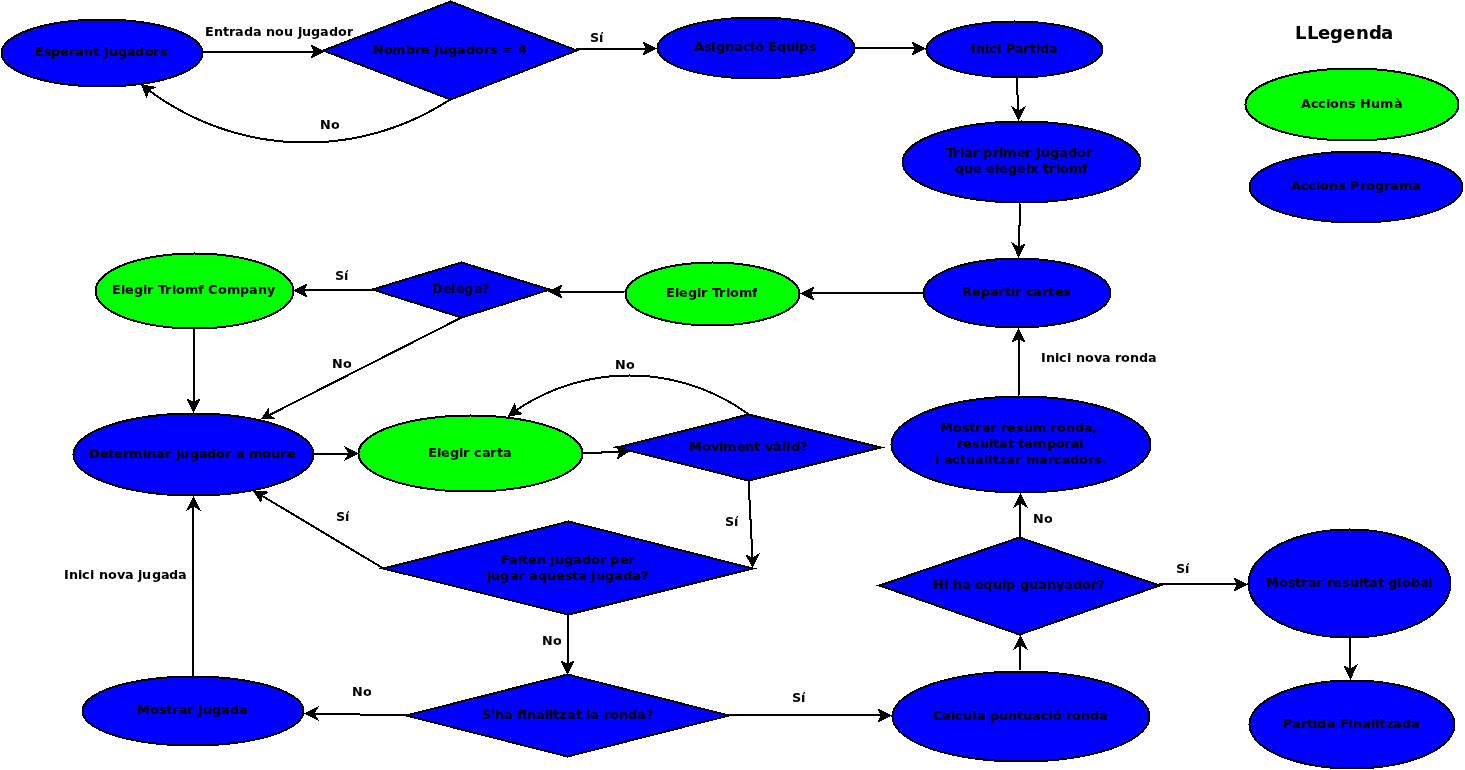
\includegraphics[width=18cm]{img/butifarra_workflow.png}
\caption{Flux de treball de la botifarra}
\label{fig:buti-workflow}
\end{figure} 

\newpage

Com es pot observar a la figura \ref{fig:buti-workflow} el servidor s'encarrega de realitzar les següents tasques referents a la botifarra: 

\begin{itemize}
\item{Començar la partida quan ja hi ha quatre jugadors. }
\item{Repartir de forma aleatòria els jugadors en dos equips. }
\item{Escollir de forma aleatòria el primer jugador en elegir triomf.}
\item{Repartir les cartes de forma aleatòria entre els diferents jugadors}
\item{Comunicar el triomf elegit a tots els jugadors.}
\item{Comunicar als jugadors si hi ha algun jugador que contrar.}
\item{Determinar el jugador a moure i notificar-l'hi de que és el seu torn.}
\item{Validar que la carta jugada és correcta.}
\item{Mostrar les cartes de cada jugada.}
\item{Al final de cada ronda mostrar el resultat parcial de la ronda. }
\item{Al final de cada ronda calcular la puntuació de cada equip. En el cas que hi hagi un equip guanyador finalitzar la partida. En el cas que no hi hagi cap jugador guanyador inicial una nova ronda.}
\end{itemize}

Tota la lògica de la botifarra s'ha realitzat en funció d'esdeveniments, és a dir, cada vegada que es produeix un acció que requereix la intervenció del servidor aquest llança un esdeveniment que té associada una funció. Aquesta funció es l'encarregada de realitzar tot el processament i llençar el pròxim esdeveniment en cas de que sigui necessari.  


\subsubsection{Aleatorietat}

Un punt molt important per a què els jugadors disfrutin de la seva partida de la botifarra és l'aleatorietat del repartiment de les cartes. Per garantir aquesta aleatorietat s'ha implementar l'algorisme de Knuth Fisher Yates\footnote{\url{http://en.wikipedia.org/wiki/Fisher-Yates_shuffle}} que permet la generació d'una permutació aleatòria sobre un conjunt finit. En el nostre cas el nostre conjunt finit es correspon amb les 48 cartes de la baralla espanyola utilitzades per jugar a la botifarra. 

Donat un conjunt de nombre de 1 a N, aquest algoritme s'aplica de la següent forma: 
\begin{enumerate}
\item{Escriure els nombre de 1 a N.}
\item{Agafar un nombre aleatori k entre 1 i el nombre d'elements pendents de tractar (inclusiu)}
\item{Contant per la part més baixa, treure el número de la posició k que encara no s'ha tractat i escriure'l a un altre lloc}
\item{Repetir el segon pas fins que s'hagin tractat tots els nombres}
\item{El conjunt de nombres que s'han escrit al pas 3 es una permutació aleatòria del conjunt de nombres inicials}
\end{enumerate}

Aquest algorisme te un cost $O(n^2)$ per això s'ha utilitzat la variant de Knuth que permet optimitzar l'algorisme fins a obtenir un cost de $O(n)$. Aquesta variant el que fa es moure els elements pendents de tractar al final de lla llista. Així l'algorisme es queda expressat de la següent forma: 

\begin{lstlisting}
 Per ordenar un conjunt de n elements (indexs 0..n-1):
   Per cada i de n \item{1 fins a 1 fer:
        j <\item{nombre aleatori que compleix que  0 <= j <= i
        canviar a[j] i a[i]
\end{lstlisting}

A més a més per tal de garantir la complerta aleatorietat i evitar possibles resultats iguals aquest algorisme s'aplica 12 vegades. Amb això s'intenta emular el comportament humà al barrejar la baralla de cartes, ja que quan es juga una partida les cartes es barrejen un nombre aleatori de vegades amb l'objectiu de que aquestes surtin el més barrejades possible. 

\section{Client}

El client s'encarrega de realitzar les següents tasques: 

\begin{itemize}
\item{Interaccionar amb el servidor a través de WebSockets.}
\item{Mostrar al usuari les dades que rep del servidor.}
\end{itemize}

Aquestes funcionalitats s'han implementat de forma separada per poder garantir que els canvis a la interfície d'usuari no afectin al la interacció amb el servidor. Aquesta separació ens permet canviar la forma en que es mostren les dades sense tenir que realitzar cap modificació a la lògica del client. Això també ens permet disposar de dos interfícies d'usuari (una per equips d'escriptori i l'altra per a mòbils, per exemple) que utilitzen els mateixos mecanismes per tal d'interactuar amb el servidor. 

En els següents apartats s'explica com s'han implementat aquestes dues funcionalitats. 

\subsection{Lògica del client}

Per tal d'implementar la comunicació entre el client i el servidor s'ha utilitzat la llibreria socket.io. Aquesta llibreria proporciona els mètodes necessaris per la comunicació entre client servidor. Aquest és el mètode emprat en la nostra implementació. A través d'aquest fitxer JavaScript obtenim els mètodes suficients per connectar-nos al servidor i poder enviar/rebre missatges. En el nostre cas el client proporciona els mètodes per poder interaccionar amb el servidor i obtenir tota la informació comentada en la secció \ref{sec:interconnexio-jugadors}. A més a més s'encarrega d'escoltar els següents següents missatges: 

\begin{description}
\item[welcome]{Missatge de benvinguda del servidor.}
\item[message]{Rep els missatges enviats per altres jugadors.}
\item[updated-game]{Informa sobre l'actualització d'informació d'una partida. }
\item[start]{Una partida que l'usuari es jugador comença.}
\item[select-thriumph]{Informa al jugador que ha de seleccionar el trumfo de la partida. }
\item[notify-thriumph]{Informa al jugador el trumfo seleccionat pels altres jugadors.}
\item[play-card]{El jugador ha de seleccionar una carta per jugar. }
\item[played-card]{S'ha jugat una carta.}
\item[new-move]{Comença una nova basada.}
\item[end-move]{S'ha finalitzat la basada activa.}
\item[contro]{El jugador té la possibilitat de contrar.}
\item[contro-done]{Informa que un altre jugador ha contrat.}
\item[round-ended]{S'ha finalitzat la ronda.}
\item[game-ended]{S'ha finalitzat la partida.}
\end{description}

Cada vegada que es rep un missatge d'aquest tipus el programa client s'encarrega de processar la informació i de cridar al programa de visualització de la informació\footnote{Veure secció \ref{sec:visualitzacio-informacio}} per a que mostri la informació a l'usuari. El programa client també s'encarrega de refrescar la informació del servidor de forma periòdica. 




\section{Exemples de comunicació}

En aquest apartat es mostraran alguns exemples de la comunicació que es dur a terme entre el client i el servidor, detallant els missatges que s'intercanvien. 

\begin{figure}[ht!]
\centering
\begin{sequencediagram}
\newthread[white]{c}{Client}
\newinst[9]{s}{Servidor}
 
\begin{call}{c}{Establir connexió}{s}{welcome}
\end{call}

\begin{call}{c}{login}{s}{Informació del usuari}
\end{call}

\begin{call}{c}{new-game}{s}{Informació de la partida creada}
\end{call}

\end{sequencediagram}
\caption{Diagrama de flux de creació d'una nova partida.}
\label{diag:creacio-nova-partida}
\end{figure} 

A la figura \ref{diag:creacio-nova-partida} es pot observar el diagrama de flux necessari per a la creació d'una nova partida. En el primer pas el programa client estableix la connexió amb el programa servidor que li contesta donant-li la benvinguda al servidor i preguntant-li el seu nom d'usuari. Una vegada el programa client envia el nom d'usuari el programa servidor li contesta amb l'identificador usuari que te assignat. Una vegada s'ha identificat el programa 


\begin{figure}[ht!]
\centering
\begin{sequencediagram}
\newthread[white]{c}{Client}
\newinst[9]{s}{Servidor}
 
\begin{call}{c}{Establir connexió}{s}{welcome}
\end{call}

\begin{call}{c}{login}{s}{Informació del usuari}
\end{call}

\begin{call}{c}{list-games}{s}{Llista de partides}
\end{call}

\begin{call}{c}{join-game(id)}{s}{Confirmació.}
\end{call}

\end{sequencediagram}
\caption{Diagrama de flux per entrar a una partida existent.}
\label{diag:entrar-partida}
\end{figure} 

A la figura \ref{diag:entrar-partida} es pot observar el diagrama de flux necessari per a la creació d'una nova partida. En el primer pas el programa client estableix la connexió amb el programa servidor que li contesta donant-li la benvinguda al servidor i preguntant-li el seu nom d'usuari. Una vegada el programa client envia el nom d'usuari el programa servidor li contesta amb l'identificador usuari que te assignat. Una vegada s'ha identificat el programa 

\begin{figure}[ht!]
\centering
\begin{sequencediagram}
\newthread[white]{s}{Servidor}
\newinst[9]{c}{Client}
 
\begin{messcall}{s}{start-game(game-data)}{c}
\end{messcall}

\begin{sdblock}{ Ronda } { Mentre no hi hagi equip guanyador.}

   \begin{call}{s}{select-thriumph(choises)}{c}{made-thriumph(thriumph)}
    \end{call}

    \begin{messcall}{s}{chosen-thriumph(thriumph)}{c}
    \end{messcall}

    \begin{call}{s}{contro}{c}{do-contro(value)}
    \end{call}

    \begin{messcall}{s}{new-move)}{c}
    \end{messcall}

    \begin{sdblock}{ Jugada } { Fins que no quedin cartes per jugar }
        
        \begin{messcall}{s}{play-card}{c}
        \end{messcall}
        
        \begin{messcall}{c}{new-roll}{s}{missatge-error}
        \end{messcall}
        
        \begin{messcall}{s}{played-card}{c}
        \end{messcall}    
        
    \end{sdblock}

    \begin{messcall}{s}{end-move)}{c}
    \end{messcall}

\end{sdblock}
 
\begin{messcall}{s}{end-game(game-data)}{c}
\end{messcall}

\end{sequencediagram}
\caption{Diagrama de flux del desenvolupament d'una partida.}
\label{diag:desenvolupament-partida}
\end{figure} 


A la figura \ref{diag:desenvolupament-partida} es pot observar el diagrama de flux del desenvolupament d'una partida. En aquest cas s'han omès els passos de creació d'una nova partida i que cada jugador entri dins de la partida. La partida comença quan el servidor notifica a tots els jugadors de la partida que aquesta ha començat. Durant el transcurs de la partida es van jugant diferents rondes. En cada ronda el servidor notifica al client que ha de seleccionar thriumph les opcions que té diferent i espera la resposta del client. Una vegada el client ha seleccionat triomf, notifica a tots els jugadors de la partida quin ha estat el triomf seleccionat. Després d'això, notifica als jugadors que tenen la possibilitat de contrar i espera la seva resposta. Una vegada s'ha realitzat el proces de contro, el servidor indica el començament d'una nova jugada amb el missatge new-move. Cada jugada consisteix en un moviment (nova carta jugada) de cadascun dels jugadors de la partida. Així per cada moviment del jugador el servidor notifica al client que ha de realitzar un nou moviment i espera rebre el missatge de que s'ha jugat una nova carta. Quan el client envia el missatge de que vol jugar una nova carta el servidor valida que el moviment sigui correcte. En el cas de que aquest sigui incorrecte ho notifica al client i espera la jugada d'una nova carta. En el cas contrari, notifica a la resta de jugadors la carta que s'ha jugat i repeteix de nou la jugada. Així es van produint jugades fins que s'han acabat totes les cartes de tots els jugadors, concretament es tracta de 12 jugades. Una vegada s'han jugat totes les cartes la ronda es dona per finalitzada i el servidor computa les puntuacions de la partida. En el cas que no s'hagi finalitzat la partida es comença la ronda i es torna a repetir tot el procediment realitzat anteriorment. Si hi ha un equip guanyador la partida es dona per finalitzada i es notifica a tots els clients. 


\begin{figure}[ht!]
\centering
\begin{sequencediagram}
\newthread{s}{Servidor}
\newinst{ja}{Jugador A}
\newinst{jb}{Jugador B}
\newinst{jc}{Jugador C}
\newinst{jd}{Jugador D}

%%%%%%  Torn jugador 1  %%%%
\begin{messcall}{s}{play-card}{ja}
\end{messcall}

\begin{messcall}{ja}{new-roll(card)}{s}
\end{messcall}

\begin{messcall}{s}{played-card(card,player)}{jb}
\end{messcall}

\begin{messcall}{s}{played-card(card,player)}{jc}
\end{messcall}

\begin{messcall}{s}{played-card(card,player)}{jd}
\end{messcall}
%%%%%%  FI Torn jugador 1  %%%%

\end{sequencediagram}
\caption{Diagrama de flux d'una jugada amb 4 jugadors.}
\label{diag:jugada-4-jugadors}
\end{figure} 

\newpage

A la figura \ref{diag:jugada-4-jugadors} es pot observar les interaccions entre el client i el servidor que es duen a terme per realitzar una jugada. Aquest detall es correspon amb el block \emph{Jugada} de la figura \ref{diag:desenvolupament-partida}. Així per cada jugada es realitzen els següents pasos: 

\begin{enumerate}
    \item{El servidor notifica al jugador en qüestió que és el seu torn.}
    \item{El jugador elegeix la carta que vols jugar i ho notifica al servidor.}
    \item{Si la jugada no és correcta el servidor ho notifica al jugador i espera que elegixi una nova carta.}
    \item{Si la jugada és correcta el servidor notifica als altres jugadors la carta que s'ha tirat i qui ha estat el jugador l'ha tirat.}
\end{enumerate}


\section{Iteracions Realitzades}

Com s'ha comentat al capítol \ref{chap:metodologia} per la implementació del projecte s'ha utilitzat la metodologia iterativa. En aquest apartat es detalla les iteracions que s'ha realitzat en el transcurs del projecte i les funcionalitats que s'han incorporat en cadascuna d'elles. 

\begin{itemize}
\item{Versió 0.0.1, publicada el 11/01/2012:
    \begin{itemize}
        \item{Creació d'un servidor web utilitzant express.}
        \item{Afegir comunicació bàsica entre client i servidor.}
        \item{Afegir interfície d'usuari bàsica.}
    \end{itemize}
}
\item{Versió 0.0.2, publicada el 01/03/2012: 
    \begin{itemize}
        \item{Implementació de la lògica de la botifarra.}
        \item{Afegir suport per la cobertura del codi (code coverage)}
        \item{Afegir un control per saber els jugadors que estan pendents de contrar.}
        \item{Eliminar el llançament d'errors. A partir d'ara els errors es gestiones a través de callbacks.}
        \item{Millores de la documentació.}
        \item{Implementació de l'intercanvi de missatges entre jugadors.}
        \item{Mostrar els usuaris i les partides creades al servidor.}
        \item{El servidor inicia automàticament la partida quan hi ha suficients jugadors.}
        \item{Permetre als jugadors entrar a una partida.}
        \item{Afegir una pantalla per la creació de noves partides.} 
        \item{Afegir una pantalla per a que l'usuari s'identifiqui.}
    \end{itemize}
}
\item{Versió 0.0.3, publicada el 19/03/2012: 
    \begin{itemize}
        \item{Mostrar als jugadors si el trumfo ha estat delegat o no.}
        \item{Netejar les cartes jugades de forma automàtica al cap de tres segons.}
        \item{Mostrar la puntuació total de la partida a la interfície d'usuari.}
        \item{Traducció dels joc a diferents idiomes (Català,Castellà,Anglès).}
        \item{Nous testos per millorar la cobertura del codi.}
    \end{itemize}
}
\item{Versió 0.0.4, publicada el 12/04/2012: 
    \begin{itemize}
        \item{Millora de les traduccions.}
        \item{Afegir jugadors automàtics (robots).}
        \item{Afegir estils a la interfície d'usuari. }
        \item{Quan el trumfo es botifarra multiplicar la puntuació per dos.}
        \item{Afegir les puntuacions parcials del joc a la interfície client.}
        \item{Mostrar la puntuació de la ronda cada vegada que se'n finalitza una.}
        \item{Documentar els events de fi de ronda i fi de joc de la API del client.}
        \item{Millorar els testos per cobrir més d'una ronda de joc.}
    \end{itemize}
}
\item{Versió 0.0.5, publicada el 20/04/2012:
    \begin{itemize}
        \item{Els robots juguen les cartes que el servidor els hi suggereix.}
        \item{El servidor suggereix les cartes vàlides quan el jugador juga una carta incorrecta.}
        \item{Millores en la lògica del jugadors automàtics.}
    \end{itemize}
}
\item{Versió 0.0.6, publicada el 02/05/2012:
    \begin{itemize}
        \item{Permetre que els jugadors automàtics puguin jugar sense l'us d'un WebSocket.}
        \item{Preparar el desplegament a Heroku.}
        \item{Eliminar el directori src}
        \item{Correcció d'errors en la gestió de memòria a la part del servidor.}
        \item{Es poden visualitzar partides d'altres jugadors.}
    \end{itemize}
}
\item{Versió 0.0.7 (pendent de publicar):
    \begin{itemize}
        \item{Millorar el suggeriment de cartes per part del servidor.}
        \item{Correcció d'errors JavaScript a la part del client.}
        \item{Tornar a obrir el pantalla de trumfo si no se n'ha seleccionat cap. }
        \item{Afegir una pàgina amb les estadístiques del servidor}
    \end{itemize}
}
\end{itemize}

\section{Jocs de proves}

Com s'ha comentat a l'apartat \ref{sec:tdd} per la implementació d'aquest projecte s'han utilitzat jocs de proves. En aquest apartat es detalla els jocs de proves que s'han implementat. Els testos implementats s'estructuren en dos blocs: 

\begin{description}
    \item[Botifarra]{ Són els testos encarregats que la lògica de la botifarra es compleixi a la perfecció.}
    \item[Comunicació client-servidor] {Jocs de proves encarregats de validar que al comunicació entre el client i el servidor es realitza de forma correcta.}
\end{description}

L'objectiu d'un joc de proves es festejar el correcte funcionament d'una funcionalitat de l'aplicació. Executant els jocs de proves cada vegada que es realitzi una modificació a l'aplicació podem garantir que les millores implementades anteriorment no han deixat de funcionar. 

A les següents línies de codi podem observar el joc de proba que s'utilitza per assegurar-nos de que una partida de botifarra no es pot jugar amb menys de 4 jugadors. 

\begin{lstlisting}
"A butifarraGame needs 4 players to start" : function() {
    var game = Game.create();
    var player1 = Player.create('John');
    var player2 = Player.create('Mark');
    var player3 = Player.create('Steve');
    var player4 = Player.create('Bill');
    game.min_players.should.eql(4);
    should.throws(function(){
        game.start();
    },Error,"Not enough playerss");
    player1.join(game);
    player2.join(game);
    player3.join(game);
    player4.join(game);
    should.doesNotThrow(function(){
        game.start();
    },Error,"Not enough players");      
}
\end{lstlisting}

El joc de proves s'estructura de la següent forma:

\begin{description}
    \item[línies 2-6]{Inicialitzem les variables necessàries per realitzar la prova.}
    \item[línies 7-10]{Comprovem que el programa ens dona error en cas de que no hi hagi suficients jugadors.}
    \item[línies 11-17]{Comprovem que el programa no es dona error quan hi ha els suficients jugadors.}
\end{description}

A les següents línies de codi podem observar el codi necessari per validar que la primera carta d'una jugada pot ser qualsevol carta.

\begin{lstlisting}
"The first Roll of a move could be any card" : function(done){
    var CavallEspases = Card.create(11,'Espases');
    player1.cards=[CavallEspases];
    move.addRoll(player1,CavallEspases,function(err){
        should.ifError(err);
        move.rolls.length.should.eql(1);
        move.rolls[0].card.should.eql(CavallEspases);
        move.rolls[0].player.should.eql(player1);
        done();
    });
}
\end{lstlisting}

Com podeu observar aquest test es molt més simple que l'anterior, ja que l'únic que fa es jugar una carta a l'atzar, comprobar que no es produeix cap error i validar que la carta s'ha afegit correctament a la jugada.

\subsection{Botifarra}

Pel que fa a l'apartat de la botifarra podem trobar els següents jocs de proves:


\begin{itemize}
    \item{Un jugador esta composat per un nom i un correu electrònic.}
    \item{Em de ser capaços de comparar els jugadors.}
   \item{Una carta esta composada per un número i un pal.}
    \item{Hem de ser capaços de determinar si una carta es superior a una altra.}
    \item{Una baralla de cartes esta formada per 48 cartes.}
    \item{Hem de ser capaços de barrejar la baralla de cartes.}
    \item{Hem de poder obtenir una o més cartes de la baralla.}
   \item{Hem de saber les cartes que queden a la baralla.}
    \item{Els jugadors inicials d'una partida són 0.}
    \item{Es poden afegir jugadors a una partida.}
    \item{Es poden afegir observadors a una partida.}
    \item{Es poden eliminar jugador d'una partida.}
    \item{Les partides poden ser clonades.}
    \item{Hem de poder saber l'estat d'una partida.}
    \item{Després de començar una partida el seu estat és En Curs.}
    \item{El joc de la botifarra consisteix amb: jugadors, equips i puntuacions.}
    \item{Una partida requereix 4 jugadors.}
    \item{No poden jugar més de 4 jugadors en la mateixa partida.}
    \item{Després de començar la partida es crea la primera ronda.}
    \item{Després de començar la partida tots els jugadors pertanyen a un equip.}
    \item{Després de jugar una ronda s'actualitzen les puntuacions.}
    \item{Si el trumfo es botifarra les puntuacions es multipliquen per dos.}
    \item{Si un jugador ha contrat les puntuacions es multipliquen per dos.}
    \item{Quan un equip supera els 100 punts la partida s'ha acabat.}
    \item{Una jugada de la botifarra consisteix amb 4 moviments.}
    \item{Els jugadors poden afegir el seu moviment a la jugada actual.}
    \item{El primer moviment d'una jugada pot ser qualsevol carta.}
    \item{Una jugador no pot realitzar dos moviments a la mateixa jugada.}
    \item{Una carta no es pot tirar dos vegades a la mateixa jugada.}
    \item{S'ha de tirar una carta del pal inicial de la jugada o trumfo.}
    \item{Si es possible, s'ha de superar la carta de l'equip rival.}
    \item{Al finalitzar una jugada s'ha de calcular el guanyador i el valor de la mateixa.}
    \item{Un jugador només pot jugar una carta que te a la seva pila.}
    \item{Si un jugador no té cartes del pal actual ha de jugar trumfo.}
    \item{S'han de suggerir les cartes correctes en cas de que el moviment sigui invalid.}
    \item{Si un jugador no té trumfo ni cap carta del pal actual pot jugar qualsevol carta.}
    \item{Si el guanyador de la jugada és el nostre company i no tenim cap carta del pal inicial, podem jugar qualsevol carta.}
    \item{Una ronda esta formada per 12 moviments i un trumfo.}
    \item{Hem de poder saber si el trumfo s'ha delegat o no.}
   \item{Hem de poder saber les cartes que ha guanyat cada equip.}
    \item{Quan es comença la ronda, cada jugador té 12 cartes.}
    \item{Només es pot seleccionar trumfo una vegada per ronda.}
    \item{Quan és delega el company pot fer trumfo.}
    \item{Desprès de fer trumfo, es permet la possibilitat de contrar.}
    \item{Si algun jugador contra, la puntuació es multiplicarà per 2.}
    \item{Es guarda els jugadors que han contrat la ronda.}
    \item{Quan s'acaba la jugada, les cartes s'assignen a l'equip guanyador.}
    \item{S'ha de poder calcular la puntuació de la ronda.}
    \item{Una ronda consisteix en 12 jugades.}
\end{itemize}  

\subsection{Comunicació client-servidor.}

Pel que fa a l'apartat de comunicació entre el  podem trobar els següents jocs de proves:

\begin{itemize}   
    \item{Hem de ser capaços de connectar al servidor.}
    \item{Es poden realitzar més d'una connexió simultània al servidor.}
    \item{Ens hem de poder identificar amb el servidor.}
    \item{Hem de poder llistar els jugadors connectats al servidor.}
    \item{Hem de poder llistar les partides que existeixen al servidor.} 
    \item{Hem de ser capaços de crear noves partides al servidor.}
    \item{Ens hem de poder comunicar amb els altres jugadors connectats.}
    \item{Hem de poder entrar a una partida existent.}
    \item{Hem de poder veure una partida existent.}
    \item{Només es pot jugar una partida una sola vegada.}
    \item{No es pot veure una partida que s'esta jugant.}
    \item{No es pot entrar a un joc que no existeix.}
    \item{El servidor ha de respondre dels events de la ronda.}
    \item{Hem de poder afegir robots a la partida.}
    \item{El servidor ha de ser capàs de traduir els textes del joc.}
\end{itemize}

